\section{Irvan Rizkiansyah(1174043)}
	\subsection{Instalasi mapserver dan mapproxy}
		\begin{enumerate}
			\item Pertama download terlebih dahulu mapservernya pada website mapserver-nya, untuk download bisa klik \href{https://mapserver.org/} {disini}
			
			\item Kemudian extract file yang sudah di download tadi pada direktori C, gambar dibawah ini merupakan hasil yang sudah di extract.
				\begin{figure}[H]
					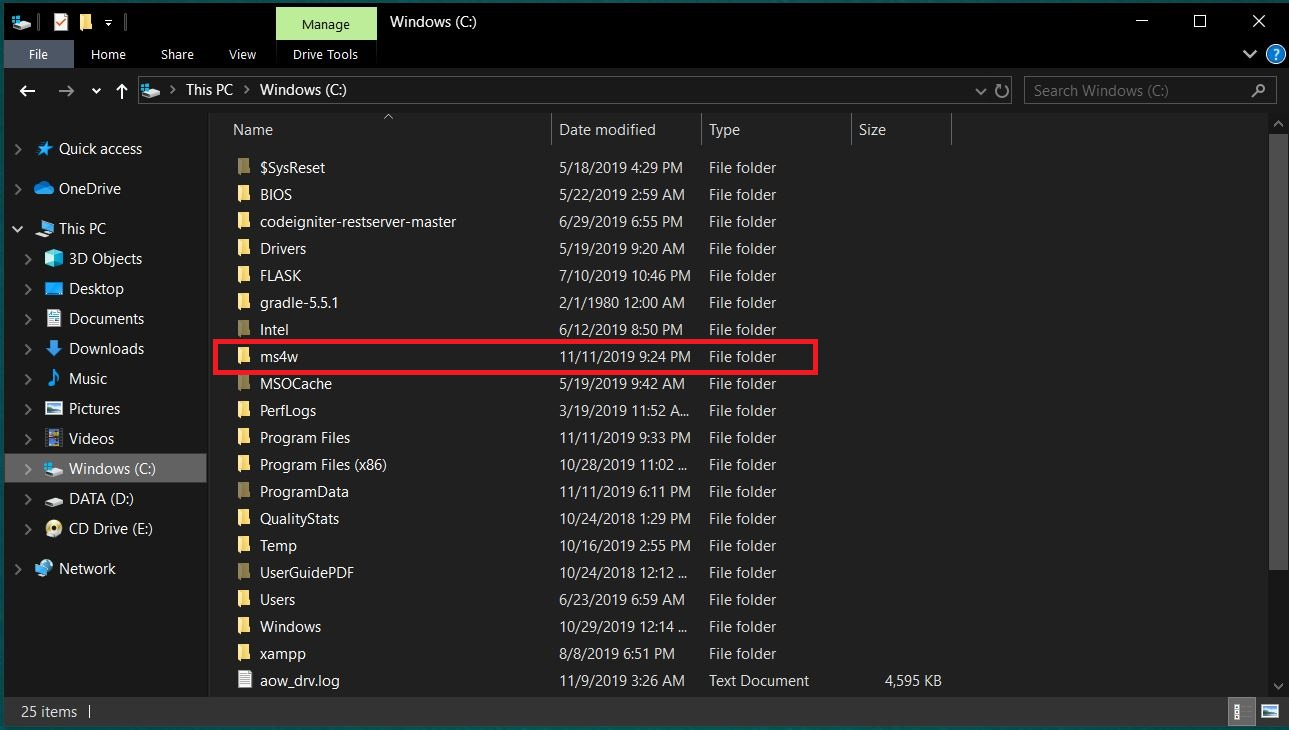
\includegraphics[width=12cm]{figures/1174043/TUGAS4/1.JPG}
					\centering
					\caption{Hasil Extract}
				\end{figure}
			
			\item Setelah itu buka Command Prompt sebagai Administrator, dan masuk ke direktori dari hasil yang sudah di extract sebelumnya dengan perintah seperti pada gambar dibawah ini
				\begin{figure}[H]
					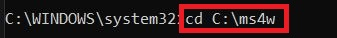
\includegraphics[width=12cm]{figures/1174043/TUGAS4/2.JPG}
					\centering
					\caption{Perintah cd}
				\end{figure}
				
			\item Kemudian jalankan file apache-install.bat dengan perintah seperti pada gambar dibawah ini
				\begin{figure}[H]
					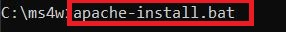
\includegraphics[width=12cm]{figures/1174043/TUGAS4/3.JPG}
					\centering
					\caption{Perintah cd}
				\end{figure}
				
			\item Jika sudah maka hasilnya akan seperti pada dibawah ini, sejauh ini mapserver sudah terinstall dan dapat dijalankan
				\begin{figure}[H]
					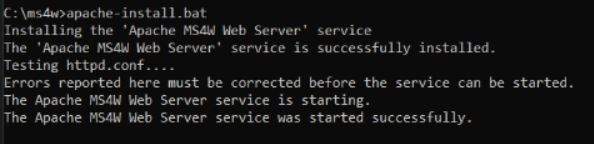
\includegraphics[width=12cm]{figures/1174043/TUGAS4/4.JPG}
					\centering
					\caption{Perintah cd}
				\end{figure}
				
			\item Kemudian kita lakukan instalasi mapproxy dengan perintah pip install mapproxy seperti dibawah ini
				\begin{figure}[H]
					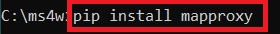
\includegraphics[width=12cm]{figures/1174043/TUGAS4/5.JPG}
					\centering
					\caption{Perintah cd}
				\end{figure}
				
			\item jika sudah melakukan instalasi mapserver dan mapproxy, kita akan mencoba dengan menggunakan peta indonesia yang sudah disediakan bisa diklik \href{https://github.com/awangga/gede} {disini}. Kemudian jalankan file 00.shp yang terdapat pada folder shp menggunakan aplikasi QGIS dan hasilnya akan seperti dibawah ini.
				\begin{figure}[H]
					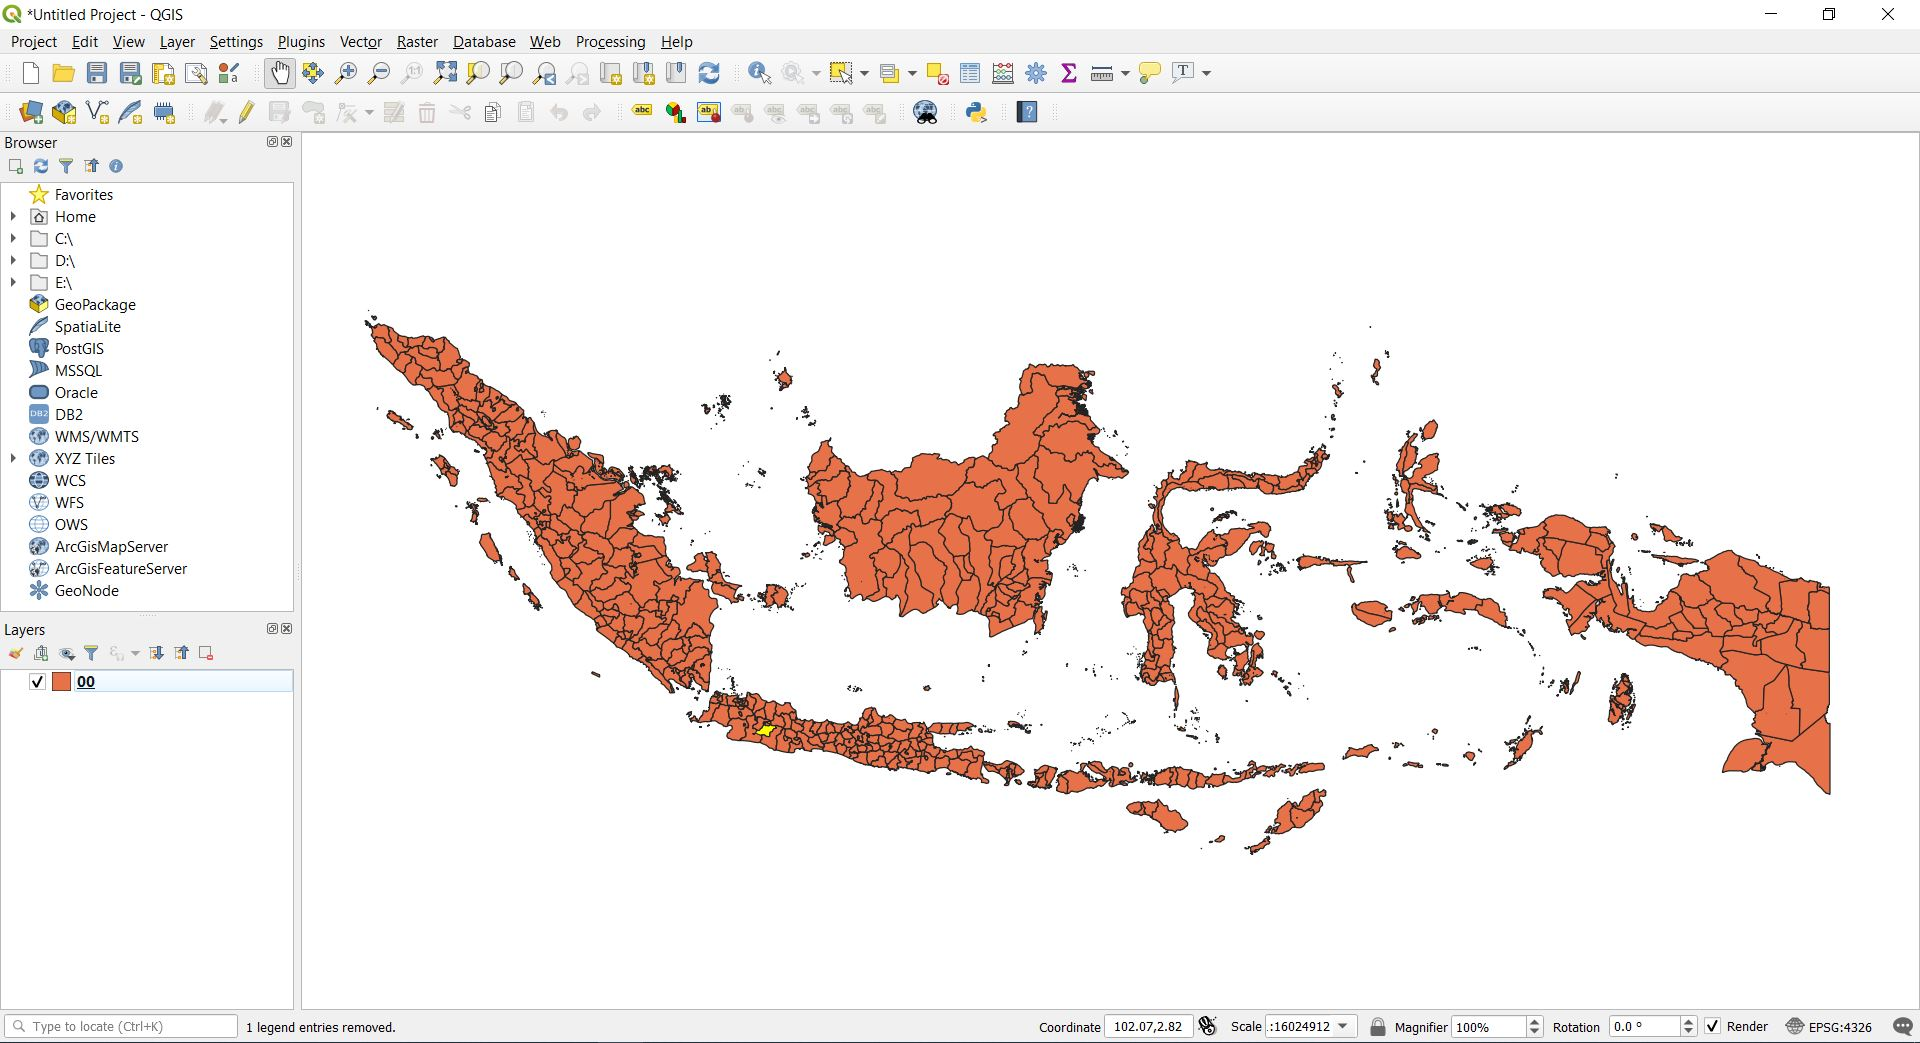
\includegraphics[width=12cm]{figures/1174043/TUGAS4/6.JPG}
					\centering
					\caption{Perintah cd}
				\end{figure}
				
		\end{enumerate}
			
	\subsection{Link video Instalasi mapserver dan mapproxy}
		\href{https://youtu.be/i0Igx8knqpQ} {Link video Instalasi mapserver dan mapproxy - Irvan Rizkiansyah - 1174043}